\documentclass{article}

% these packages let you do math
\usepackage{amsmath}
\usepackage{amssymb}

% we need these packages for fancy R tables
\usepackage{booktabs}
\usepackage{float}
\usepackage{colortbl}
\usepackage{xcolor}

% these packages play with the spacing/margins of the document. Uncomment the commands on lines 16 and 17 to see what they do.
\usepackage{a4wide}
\usepackage{setspace}
\usepackage{geometry}
\usepackage{parskip}
%\doublespacing
%\geometry{margin=1.5in}

% this package helps us with including images. Setting the graphics path makes it easier to refer to things in the \includegraphics command.
\usepackage{graphicx}
\graphicspath{ {../figures/} }

% make some hyperlinks using the \href command
\usepackage{hyperref}
\hypersetup{
    colorlinks=true,
    linkcolor=black,
    urlcolor=blue
}

% set the author, title, and date of the document. \maketitle adds it to the document.
\author{Shawn Leavor}
\title{My Paper on NLSY97 Data}
\date{February 2022}

\begin{document}
\maketitle

\section{Introduction}

Taking data from the NLSY97 on Incarceration Status, I was able to find differences in incarceration rates based on race and gender. I analyzed the incarceration status of everyone for the year of 2002 and tracked the average number of months people were incarcerated for the year of 2002 based on their race and gender. Many of the survey respondents were not incarcerated at all for the year 2002, so the average months incarcerated all tend to be very low. 

We run the following regression:

\begin{equation*}
    y = \beta_1 + \beta_2 Hispanic + \beta_3 Mixed Race (Non-Hispanic)+ \beta_4 Non-Black / Non-Hispanic + \beta_5 Male + \varepsilon
\end{equation*}

\section{Analysis}

Wherein we do tables and graphs. To include the graph we made in ggplot, we create the \texttt{figure} environment. The `H' option tells LaTeX to `hold' the position of the figure instead of positioning it somewhere else. I use the \texttt{caption} command to add a caption{\textemdash}although I also put a title on the plot in ggplot so you would typically choose one or the other. I use the \texttt{label} command after the caption to add a label. Then in my paper I can use the \texttt{ref} command and LaTeX knows I am referring to Figure \ref{fig:graph}.


\begin{figure}[H]
    \begin{center}
        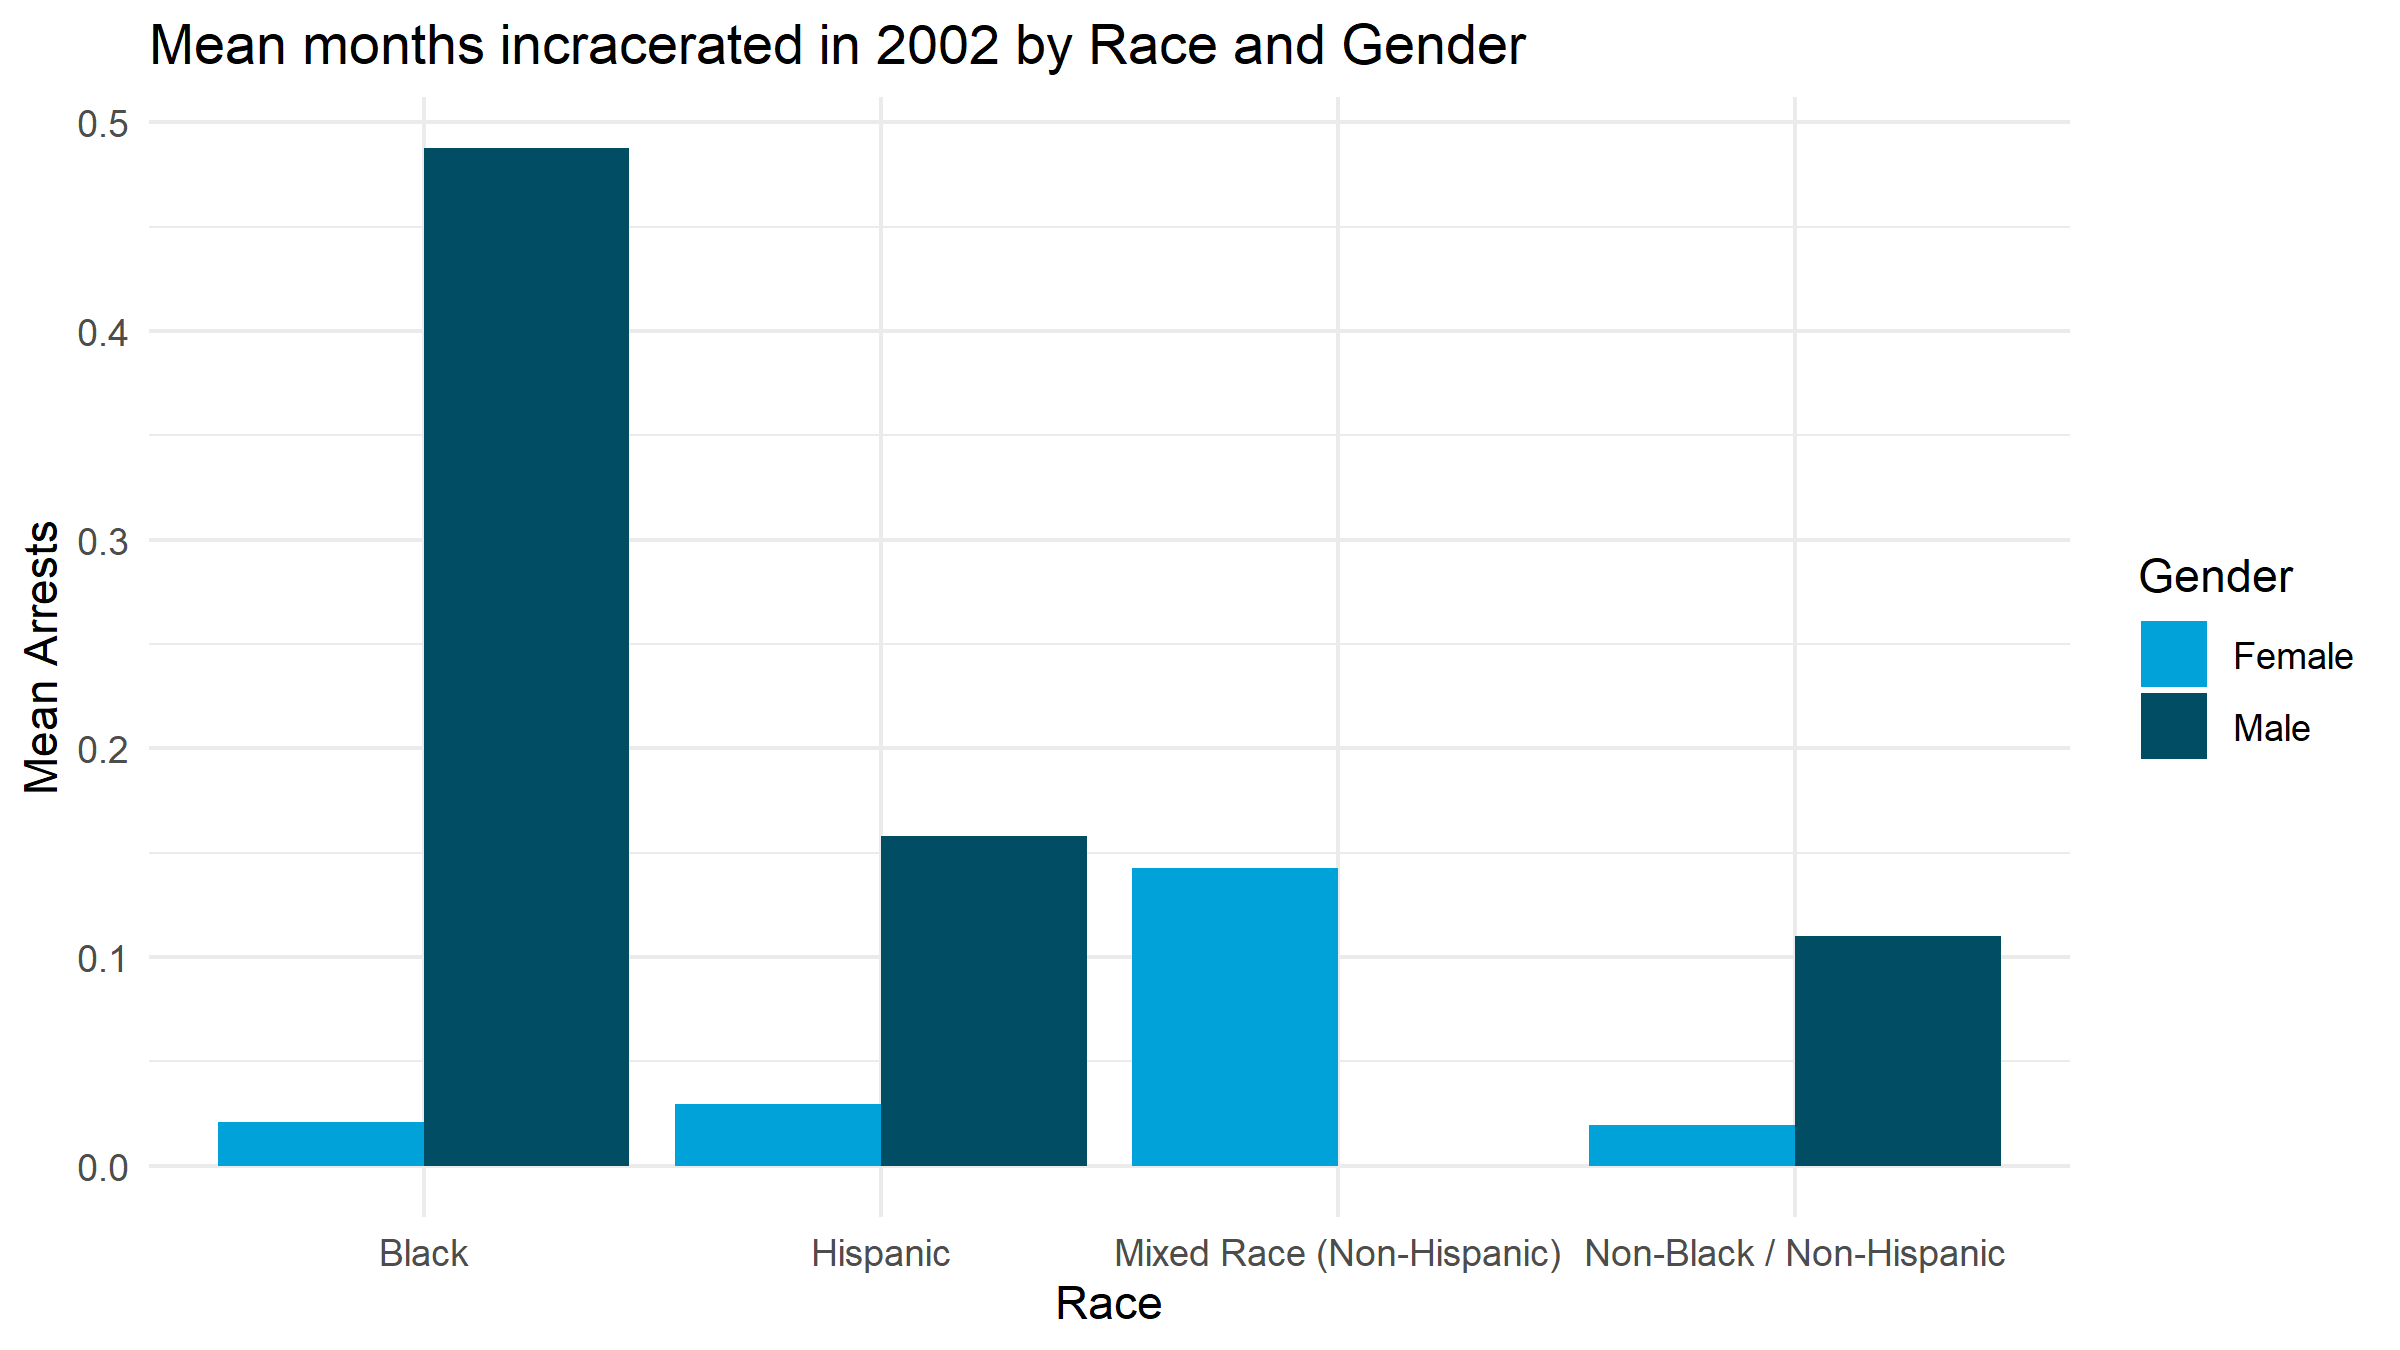
\includegraphics[width=.85\textwidth]{arrests_by_racegender}
    \end{center}
    \caption{Mean Number of Months Incarcerated in 2002 by Race and Gender}
    \label{fig:graph}
\end{figure}

The above graph shows the mean number of incracerations in 2002 based on race and gender. We see in every category except for Mixed Race (Non-Hispanic) that the mean number of incarceration months is higher for males than for females. We also see that this rate is much higher for black males than any other category. Interestingly, we see that male mixed race Non-Hispanic has an average incaceration months of 0. 

\begin{table}[H]

\caption{\label{tab:tab:summarystats}Mean months incracerated in 2002 by Race and Gender}
\centering
\begin{tabular}[t]{lrrrr}
\toprule
Gender & Black & Hispanic & Mixed Race Non Hispanic & Non Black Non Hispanic\\
\midrule
\cellcolor{gray!6}{Female} & \cellcolor{gray!6}{0.0211268} & \cellcolor{gray!6}{0.0298013} & \cellcolor{gray!6}{0.1428571} & \cellcolor{gray!6}{0.0193192}\\
Male & 0.4876712 & 0.1579509 & 0.0000000 & 0.1099476\\
\bottomrule
\end{tabular}
\end{table}


Table 1 is a numeric representation of Figure 1. This confirms that Black males spend the most average months incarcerated, while mixed race Non-Hispanic males spent no time incarcerated in 2002.


% Table created by stargazer v.5.2.2 by Marek Hlavac, Harvard University. E-mail: hlavac at fas.harvard.edu
% Date and time: Mon, Jan 31, 2022 - 5:56:22 PM
\begin{table}[!htbp] \centering 
  \caption{Regression Output. Omitted category is Black Females.} 
  \label{tab:regression} 
\begin{tabular}{@{\extracolsep{5pt}}lc} 
\\[-1.8ex]\hline 
\hline \\[-1.8ex] 
 & \multicolumn{1}{c}{\textit{Dependent variable:}} \\ 
\cline{2-2} 
\\[-1.8ex] & Months incracerated in 2002 \\ 
\hline \\[-1.8ex] 
 Hispanic & $-$0.159$^{***}$ \\ 
  & (0.038) \\ 
  & \\ 
 Mixed Race (Non-Hispanic) & $-$0.174$^{**}$ \\ 
  & (0.083) \\ 
  & \\ 
 Non-Black / Non-Hispanic & $-$0.189$^{***}$ \\ 
  & (0.035) \\ 
  & \\ 
 Male & 0.194$^{***}$ \\ 
  & (0.022) \\ 
  & \\ 
 Constant & 0.155$^{***}$ \\ 
  & (0.026) \\ 
  & \\ 
\hline \\[-1.8ex] 
Observations & 8,621 \\ 
R$^{2}$ & 0.015 \\ 
Adjusted R$^{2}$ & 0.014 \\ 
Residual Std. Error & 1.019 (df = 8616) \\ 
F Statistic & 32.033$^{***}$ (df = 4; 8616) \\ 
\hline 
\hline \\[-1.8ex] 
\textit{Note:}  & \multicolumn{1}{r}{$^{*}$p$<$0.1; $^{**}$p$<$0.05; $^{***}$p$<$0.01} \\ 
\end{tabular} 
\end{table} 


Table 2 is the result of a regression that shows the effects of race and gender based on the regression in Section 1. We find that the squared correlation is only 0.015 showing a poor fit of race and gender to the number of months incarcerated. However, we find that each of our p-values is significant, which tells us that race and gender have a large effect on the number of months incarcerated. On average, being male will increase the number of months incarcerated in 2002 by 0.194. We can also see that Black is the biggest factor in race, since it is the omitted variable and the other races have negative values. Our constant represents the average number of months incarcerated for a Black female. 





\end{document}